\documentclass[../main/main.tex]{subfiles}

\newdate{date}{07}{05}{2020}

\begin{document}

\renewcommand\vec{\mathbf}

\section{Lecture 18}
\displaydate{date}.  Compiled:  \today. Rachele 

\subsubsection{Slide 292}

\begin{figure}[h!]
\centering
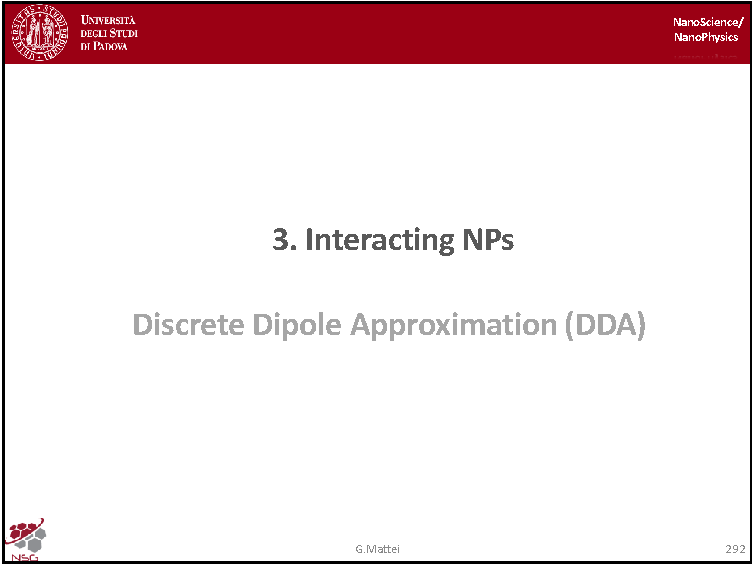
\includegraphics[page=1,width=0.9\textwidth]{../lessons/pdf_file/18_lesson.pdf}
\end{figure}


The technique we have seen to obtain an effective medium description of a material composed by an array of randomly distributed dipoles within a matrix, lead us to the development of an effective dielectric function which is able to describe composite materials (metamaterials) as an homogeneous medium with peculiar properties obtained by suitable combination of the two dielectric functions.
This concept can be generalized in a very clever way to deal with another class of problem in which interaction is very important. 

If we want to to calculate the optical properties of randomly shaped objects of course the high symmetry of the Mie theory or the Gans theory, with their spheres and spheroidal particles respectively, is no longer suitable to be to be used. We need to find some other technique for dealing with these complex shaped objects.
A unified concept which deals with both interacting dipoles and complexly shaped nanoparticles is the Discrete Dipole Approximation or DDA, which is a simple technique and we will use it also for doing some simulations in the lab activities.

\newpage

\subsubsection{Slide 293}

\begin{figure}[h!]
\centering
\includegraphics[page=2,width=0.9\textwidth]{../lessons/pdf_file/18_lesson.pdf}
\end{figure}

Suppose that we want to calculate the optical properties of an object which is quite large with respect to the wavelength or is of the same size of the wavelength and suppose for simplicity that we are dealing with a sphere.
Of course we cannot read this sphere globally in the dipolar approximation.
On the contrary we want to subdivide the volume of the original particle (which in this case is a sphere but it could be any arbitrarily shaped object) into subvolumes and we assigne to each of these subvolumes a dipole moment, as you can see in this picture here, so that we have a sort of an atomistic decomposition of our continuously shaped object into a discrete set of dipoles which are so close that they cannot be considered as independent dipoles so we need to consider the interaction between neighbouring dipoles and all the other dipoles and we would like to have a sufficiently high number of dipoles so that this discretization of the shape can be a good representation of the global properties of the entire object.
Let's suppose to have a subdivision into N number of discrete dipoles labelled by $j$.
We assign a spatial coordinate to each of those dipoles $\vec{r}_j$ and a polarizability which can be the  expression that we find with the Clausius-Mossotti the or in the Maxwell-Garnett or in the Mie theory in the dipolar approximation.
We can generalize this expression to include also the presence of an external medium in the system, but let's assume that we are in vacuum.
If we are within the material this interaction is true, because within the material each dipole is described by the dielectric function of the material, but the medium in between the dipoles can be considered the vacuum, so that this approximation holds.

We have interacting dipoles, because they are very close to each other (in the $\alpha_j^{CM}$ formula, $d$  is the local diameter of the equivalent cubic volume that we have assigned to each dipole, it’s the cube root of the entire volume of the object divided by the number of dipoles).
Now let's suppose to shine a plane wave $\vec{E}_{inc,j}$ on the system.
It is calculated at the coordinate $\vec{r}_j$ so we know what is the value of the incident field at the level of $\vec{r}_j$ dipole.
But of course, since that we have interacting dipoles, the field at the coordinate $j$ is not only the plane wave but it's also the field scattered by all the other induced dipole moments $\vec{P}_j$ in all the other coordinates.

The equation that we can write is that the induced dipole moment is proportional to the local field $\vec{E}_j$ times the polarizability of the dipole $\alpha_j$. 
We need to calculate the local field at the $j$ coordinate: it is the sum of the incident field plus the contribution of all the other dipoles but the $j$ one $\vec{P}_k$ with the suitable phase functions which describe the distance and the effect of the dipole at the distance $\vec{r}_{jk}$  which is the modulus of the difference in the distance between $\vec{r}_{j}$ and $\vec{r}_{k}$ dipoles.  $\hat{r}_{jk}$  is the unitary vector in that direction.

 The elements of the matrix $\vec{A}_{jk}$ come from the simple theory of the dipole interaction with respect to a given distance and a given direction, so this is a definition, even if a bit complex. $\vec{A}_{jk}$ are built by the relative distance and relative phase of the dipole moments at the two coordinates.
We define the diagonal elements, instead, as the inverse of the polarizability of the $j$ dipole.
So we can build a square matrix N by N, which is well defined in all the elements, and we can recast the equation for $\vec{E}_{j}$ into a system in which we have the sum of $k$ from 1 to N of the $jk$ element of the matrix times the induced dipole $\vec{P}_{k}$ equal to the incident field calculated in the $j$ coordinate.
This is a self consistent way to deal with the field at each dipole by including the effect of all the other dipoles in the system (because we are in the interacting approximation for the dipoles).

\newpage

\subsubsection{Slide 294}

\begin{figure}[h!]
\centering
\includegraphics[page=3,width=0.9\textwidth]{../lessons/pdf_file/18_lesson.pdf}
\end{figure}

The problem is now to solve those kind of a problems in which we can use the matrix notation.
We can rewrite the entire problem in the very compact form $\vec{ \widetilde{A}} \vec{ \widetilde{P}} = \vec{ \widetilde{E}}_{inc}$ in which the vector $\vec{ \widetilde{P}}$ is the list of all the vectors of the induced dipoles in the system, the matrix $\vec{ \widetilde{A}}$ contains all the terms that we need and the vector $\vec{ \widetilde{E}}_{inc}$ is a column vector with N components of the value of the planewave at the coordinate $\vec{r}_j$ of each dipole.
Of course there are well known techniques for inverting this matrix and find the solution of this homogeneous system.
We can solve for the values of $\vec{ \widetilde{P}}$, which are our unknowns, and from those we can write the extinction and the absorption cross-section and we can calculate the scattering field produced by the entire array of the objects.
So, in this way, we can compute all the properties that we need to have information on the scattered field, the absorption, the extinction and of course the scattering cross-section by just subtracting the first from the second one.
With this technique of course we can obtain a suitable approximation which can be tested respect to the Mie theory which is exact for spheres. We can also have an estimation on how many dipoles we need to obtain an accurate description of the far field and near field properties of our system as a function of the number of dipoles.
 That is an issue of such kind of approximation, because you need to do some experiments to test the convergency of the entire process with respect to the increase of the number of dipoles.

Such kind of approximation normally is good for materials in which the refractive index is not so high or not so different from the one of typical dielectrics. For metals, since the real part of $\epsilon$ is quite large at optical frequency the level of agreement is not that satisfactory, unless we use a very large number of dipoles.
We can test the results for simply shaped objects like spheres toward the exact value that we know from the Mie theory or for ellipsoid from the Gans theory.
This theory can be used to describe not only a single object, but also an array of objects, with a bunch of dipoles describing the first object and then another bunch of dipoles describing the second object… So we can have an interaction between to metaobjects which are our nano-particles: we can discuss the interaction between dimers or with any arbitrary array of nanoparticles.
Generalize this description to any arbitrary array of objects with arbitrary shape it’s only a matter of computational power.

\newpage

\subsubsection{Slide 295}

\begin{figure}[h!]
\centering
\includegraphics[page=4,width=0.9\textwidth]{../lessons/pdf_file/18_lesson.pdf}
\end{figure}

The concept of interacting nanoparticles is very far reaching: a dimer is able to focus the external light in the gap region between the two nanoparticles, the so-called hotspots of the electric field, so we can obtain a very large field amplification in sub-wavelength domains, which is a really remarkable result.

In general, ordered arrays of nanoparticles exploit this specific interaction between nanoparticles in a very clever way, in particular in 2D settings.
If we are able to produce ordered arrays of complexly shaped nanoparticles in 2D, we add another degree of freedom in the system and we can obtain a sort of a plasmonic lattice, which exhibits band structures like normal periodic structures (and obey to the dispersion law). 

\newpage

\subsubsection{Slide 296}

\begin{figure}[h!]
\centering
\includegraphics[page=5,width=0.9\textwidth]{../lessons/pdf_file/18_lesson.pdf}
\end{figure}

In our group we are strongly investigating 2D arrays deposited on surfaces obtained with nanosphere lithography, which is a very simple lithographic technique in which we can produce ordered arrays of areas as large as centimetre squared.
This is a typical scanning electron microscope image of such an array in a plain view. 
In this case we have a nanoprismas array, the building blocks are the bright prism, with height around 50-200 nm, according to the request of the specific application. 
The local field is strongly localised at the tips.
The symmetry is the one of a honeycomb system, so you obtain the unitary cell joining the centre of four equivalent circle (two triangles are required because the honeycomb lattice is a non-Bravais lattice and so you need to specify two points to recover the entire symmetry of the system).

\newpage

\subsubsection{Slide 297}

\begin{figure}[h!]
\centering
\includegraphics[page=6,width=0.9\textwidth]{../lessons/pdf_file/18_lesson.pdf}
\end{figure}

These graphics concern the optical properties of this array of prisms. 
It’s a simulation obtained by finite element method, that is a discretization in space and time of the Maxwell equation (in particular of the fully electrodynamic calculation of the Helmholtz equation).
We can calculate the exact solution in any system of different materials, shapes, objects and compositions.
Basically you decide the structure of your sample, you shine light on it and calculate the near and far field properties: it's a sort of brute force calculation, because it is a discretization of the entire Maxwell equations, so it's computationally quite intensive (in our group we use \textit{Consol multiphysics} programme).

What is interesting is that we can produce this map of the near field with very intense hotspots on the tips of the prisms.
If we look in the 3D graphic (where there is a unit cell), you see that you have hotspots provided that the field is aligned in the direction of joining the tips. So you can obtain very intense hotspots (colour in the scale bar are in base 10 logarithmic scale: when you see 2, you have a two orders of magnitude amplification).
If you are able to put the molecules or objects that you want to probe in close proximity of the tips, you will obtain very very intense excitation.
You can also control the level of coupling between this neighbouring prisms, so you can obtain a plasmon tuning or an even larger amplification on the hotspots in the system. We will see the advantage of having also so large hotspots not only for linear application, but also for non linear optics applications.
As regard the far field we can obtain a spectrum like the one in the graphic on top-right of the slide. We have a very complex structure of the extinction cross section. 
We can decouple and assign to specific modes of the field different resonances of our system, like in particular the one near 800 nm in wavelength is a dipolar contribution, whereas the one at 500 nm is a quadrupolar contribution. 
We can play with the field distribution in our in our system: we can obtain the whole set of near field properties from the computation of the true physical models of the spectral representation.

But those systems, if cleverly designed, are able to produce an additional set of resonances, which are the  lattice resonances (because it's like the x-rays diffraction for atoms).
The scattered field from each of those single particles is able to interfere at given directions to obtain constructive or destructive interference, so we can assign to Bragg modes or lattice modes some specific resonances.

\newpage

\subsubsection{Slide 298}

\begin{figure}[h!]
\centering
\includegraphics[page=7,width=0.9\textwidth]{../lessons/pdf_file/18_lesson.pdf}
\end{figure}

We investigated a lot this kind of properties and very recently we published this paper which is dealing with the diffractive dipolar coupling in plasmonic non-Bravais lattices. 
The honeycomb is a non-Bravais lattice in the sense that two positions are not equivalent, so you need to include both particles in the unit cell in non equivalent positions. 

\newpage
\subsubsection{Slide 299}

\begin{figure}[h!]
\centering
\includegraphics[page=8,width=0.9\textwidth]{../lessons/pdf_file/18_lesson.pdf}
\end{figure}

\begin{itemize} 
\item \textbf{image a} This is the actual SEM electronic microscope image of our structure. 
The nanoparticles, made of silver, are the rounded object deposited on a glass, so for that reason, since the substrate is a non-conductive material, when you are doing electron microscopy normally have problems with electronic charge buildup, so this is sort of shadowing effect is due to the charging effect in the substrate, that is unavoidable in this non-conducting substrate.
Superimposed to the image there is exact pattern of the geometry of our system, $d$ is the diameter of the nanoparticle. You can obtain such kind of system by the very same technique that we used for the nano prisms array, but just performing a thermal annealing, so that we can transform prisms into spheres and  obtain an array of spherical nano particles but with very same honeycomb lattice on the surface.
The side of the exagon is $L$, so we have all the geometry defined.
\item \textbf{image b}  If we look at the scattering properties of this object, we have a graph like this, in which we can recognise the localized surface plasmon resonance L-SPR and at larger wavelength we obtain this additional resonance. It’s a surface lattice resonance SLR, obtained by the constructive interference of the scattering light from each individual particle which produce a global scattering from the ordered array of lattice. SLR will be absent if the array was random and not ordered like in our case.

\item \textbf{image c}  When we have periodical structures, we can build a band structure, so we can catalogue all the resonances in terms of the lattice properties of our system. In particular in this plot here we have the band structures in our system compared to the Rayleigh anomalies or the Bragg diffractions, labelled with the Miller indexes in two dimensions of that specific kind of structure. You can clearly assign the variations of the structure in our measured system to specific contribution of the constructive or destructive interference of the scattering properties of the single object.
In this particular paper we were interested in studying the coupling in a non-Bravais system like the honeycomb one, but this concept can be generalised to any arbitrary symmetric array: whatever is the symmetry of your unit cell you can obtain surface lattice modes, provided that you have a sufficient decoupling between the plasmon resonance of the single nanoparticle with respect to the expected position of the lattice resonance.
\end{itemize}

\newpage
\subsubsection{Slide 300}

\begin{figure}[h!]
\centering
\includegraphics[page=9,width=0.9\textwidth]{../lessons/pdf_file/18_lesson.pdf}
\end{figure}

To better see the properties of the modes of the far field spectrum, in this paper with two different methods, the one on the left is with finite element methods and the one on the right with a technique which is similar to the discrete dipolar approximation, we calculated the near field distribution under the localized SPR resonances. 

The largest value of the field is around the surface of each spherical nanoparticles (as in normal surface plasmon resonance), $k$ vector is perpendicular to the plane of the image and the field is polarized horizontally, so induced the field is in the same direction. 

On the country when we have the surface lattice resonance, we expect to have a more distributed modes of the field. Indeed we have a strong contribution around the particles too, but also a sort of zig zag structures of the field, which is extended on the entire surface of our two dimensional lattice. This is a clear indication that we have an extended mode, not just the localised mode, like the typical situation in the L-SPR for the single nanoparticles.
This is a way to play with the optical properties of nanostructures by constructing metasurfaces made out of individual scattering object, arranged in suitable ordered arrays.
We can build also randomly distributed nanoparticles, in order to exploit just the single particle nature, but of course in ordered array we have periodicity, a reciprocal space, group velocity for the propagation of the modes… 
We are using this approach to investigate very interesting classes of optically active materials to produce for instance nano-lasers.

\newpage
\subsubsection{Slide 301-302}

\begin{figure}[h!]
\centering
\includegraphics[page=10,width=0.9\textwidth]{../lessons/pdf_file/18_lesson.pdf}
\end{figure}


\begin{figure}[h!]
\centering
\includegraphics[page=11,width=0.9\textwidth]{../lessons/pdf_file/18_lesson.pdf}
\end{figure}

\newpage

When we have such samples which are able to strongly confine light in very narrow region, we can obtain not only fascinating linear properties, but also very interesting non-linear response of our materials.
Normally, when we apply an electric field to a material, we can write the polarization $\vec{P}$ of that specific material as a function of the electric field times the susceptibility of first order times the epsilon zero constant: this is a linear approximation of the entire property.
If the electric field is sufficiently high, we could probe other power series of the fields (written here in a very compact but not completely rigorous way) by including the $\chi^{(2)}$, $\chi^{(3)}$ or $\chi^{(n)}$ value, which are the non-linear n-order susceptibility which needs to be included to have a fully description of the polarization properties of our system.
Typically when you deal with materials, you are in the approximation of homogeneous, isotropic and linear materials, so on the assumption you can safely stay on the first order. 

But when you are shining very powerful laser with power densities of $GW/cm^2$, you can no longer stay on the linear approximation and the induced dipole in so distorted with respect to that simply linear approximation that you need to resort to more complex description and this is done by including 2nd order 3rd or even higher order, according to the investigated phenomenon.

In particular materials, when you have $\chi^{(2)}$ effect, you can obtain second harmonic generation: you shine a light with a given frequency and you double that frequency. 
Another interesting phenomenon ss optical parametric amplification.
The 3rd order non-linearity is very important for the third harmonic generation, the equivalent of the Kerr effect (optical Kerr effect in non-linear materials), the four-wave mixing… 

One way to obtain non-linear effect is to shine a very intense laser beam on your material, but as we have seen, we have materials which are very effective in capturing and localizing light at nano scale, so we can have a very intense light amplification in our system (up to two or three orders of magnitude amplification), enough to activate non-linear effects. 
Moreover we can tune the resonance of our materials to match the wavelength of our lasers, so we can really exploit the properties of those systems.

Suppose that we have the 3rd order effect in our material and zero component of the $\chi^{(2)}$ (which is true normally for symmetry reason if we have symmetry inversion as in the case of periodic structures, because if we invert the field we should invert also the polarisation, but since it is proportional to an even power of the field, there's no chance to invert it), the first active non-linearity is the 3rd order one.
If we want to study the optical Kerr effect, we have to redefine the relative dielectric function: now it is build out of the $\chi^{(1)}$ and $\chi^{(3)}$ susceptibilities. 
If we factor out a $\vec{E}$, we obtain that the residual term is $\vec{E}^2$. If we include it in the dielectric function, we obtain an intensity dependent dielectric function, an intensity dependent refractive index $n(I)$ and an intensity dependent absorption coefficient $\alpha(I)$ (because intensity is $\vec{E}^2$).

Normally when you are dealing with linear materials you can define a frequency or wavelength dependent refractive index. But if you are in a non-linear regime, you have a refractive index which is now function of the intensity of the beam and this is a remarkable degree of freedom that you have at hand.
The same you can say for the absorption coefficient, which is no longer constant, but is now intensity dependent.

In practical terms this means that you can change actively the refractive index of your material.
Suppose that $n_2$ is a positive number (it could be either positive or negative according to the specific material), you can select the direction of refraction. In the standard Snell refraction, if you enter at a given geometry with a beam with a low intensity, you have the standard linear refraction which is controlled by $n_0$. But if you increase the intensity, so you can have a large contribution of $n_2I$, you can increase the refractive index and bend the refracted beam toward the surface normal. Basically you can change the direction of the beam by controlling its intensity. You can obtain a sort of binary logic out of this simple object, because when the beam has low intensity or is in the zero state you have standard refraction, so the beam will follow the standard Snell refraction; but if the beam has high density you can deflect it toward the normal. In this way you can have a component which can exploit binary logic: optical switching or directional coupler or any other device to control light propagation, but at a speed of the change in intensity of a beam which can be much much faster than the speed of standard transistors ( based on electron motion, which suffer by the mass and the transport properties of electrons).

In principle with non-linear materials we can obtain all optical logic systems, the equivalent of the transistors with all optical devices. Photonics is a very interesting subject of research for that:  it could provide switching or commutation between 0 and 1 state at the frequency at least three orders of magnitude larger than the fastest devices, which are the high electron mobility transistors (made out of gallium arsenide). 

We can work also on the non-linear absorption: we can use $\beta$ (which can be either positive or negative) to increase or decrease the absorption as a function of the intensity. 

It is a quite non obvious and non intuitive way of reasoning, because the larger is the intensity, the lower is the absorption.

\newpage

\subsubsection{Slide 303}

\begin{figure}[h!]
\centering
\includegraphics[page=12,width=0.9\textwidth]{../lessons/pdf_file/18_lesson.pdf}
\end{figure}


The technique that we use to measure the non-linear properties of our system is the z-scan technique.
You use the third harmonic of Nd:YAG laser, which is at 355 nm in wavelength. This will pump an OPA device which is a device able to obtain a coherent laser like line, but at a tunable wavelength. 
OPA is able to provide any wavelength from 400 nm up to 2 $\mu$m in wavelength.

Then we can shine through some attenuators and an aperture to select the beam size; a beam splitter to have a reference intensity measurement in the oscilloscope. 
Then we have a lens and the sample, which we can move back and forward in the horizontal direction, which is the z coordinate (for that reason this is called the z-scan technique).

Since this lens will focus our beam into the focal plane (the focal length is 20 cm), we have plenty of space for moving our sample, so we can have different intensity at different position in our system.

Finally we collect the light passing through the sample. 

So, instead of changing the intensity of the laser, we change the density of that specific intensity on our material. This way we have a correspondence between position and intensity and we can measure the intensity dependent refractive index and absorption coefficient.

We have two detectors to do that, so we have another beam splitter.  Half beam goes to the Open Aperture signal: this detector will measure the entire light emerging from the interaction with samples; whereas the other detector measure the Closed Aperture intensity, that is the intensity emerging on another spatially selected Iris (which select just portions of the light scatted). 
OA signal gives information on the non-linear absorption coefficient $\alpha(I)$, whereas CA carries information of the non-linear refraction $n(I)$.

The net effect that we can measure by measuring the two signals are reported in these two graphs for OA and CA respectively. 
In OA if we have $\beta>0$ we increase the absorption as a function of increasing intensity, so we expect a decrease in the transmittance. 
If we label as 0 the position at the maximum of the focal length of the lens, we will have there the maximum intensity and the less transmitted light, because we have the largest absorption. 
When the sample passes over the maximum intensity, we have this symmetric situation. 
The situation is opposite for $\beta<0$, in this case we decrease the absorption coefficient as a function of intensity and we get a maximum at the focal plane, because there we have a minimum in the absorption. 


The situation is a little bit more complicated for the CA situation.
The continuous line is for $n_2>0$, the material will act as a sort of focusing lens, because we increase the refractive index and we will have a stronger focusing of the light emerging from the samples (in $z<0$ region).
On the contrary in $z>0$ region, that is the portion of the beam seen by CA, the intensity will be spread over a larger area. So, if we have CA, that is if we select just a portion of the beam, we will see a net decrease in intensity. 
Then after the sample passes through the maximum we will have the opposite effect, because the sample is still focusing, but now it is on the same side of the detector. So we will expect more intensity focused onto the selected apertures, so we will have an increase in intensity and then a decrease when we are sufficiently at lower intensity to have recovered the linear properties.

\newpage

\subsubsection{Slide 304}

\begin{figure}[h!]
\centering
\includegraphics[page=13,width=0.9\textwidth]{../lessons/pdf_file/18_lesson.pdf}
\end{figure}

The photo shows our experimental setup: there is a  pulse laser which operates in the picosecond regime, $\Delta t$ is the pulse duration. This duration (and not a nanosecond one) is very important,  because if you are working at that regime you excite the electrons, but also the phononic system of your material. Infact the excitation is slow enough to let electrons thermalize with lattice phonons, so globally you heat up your material. 

If you heat a material you can change the refractive index, but in a thermal way, that is in a slow way.

If we want to have a very fast non-linearity which is able to switch at the speed of the change of the intensity in our material, we want to exploit the truly electronic non-linearity, in which the phononic system is frozen because is too slow to follow the fast changes occuring at the femtosecond or picosecond in the electronic system (so it would be the same also for femtosecond lasers).

We have also the issue of tunability, because we couple the laser with the OPA, which is able to obtain a excitation laser which can be scanned around the resonances. In this way we are able to obtain a spectral non-linearities, that is all those quantities as a function, not only of the intensity, but also of the frequency (which is the full information that we can obtain with this system).

\newpage

\subsubsection{Slide 305}

\begin{figure}[h!]
\centering
\includegraphics[page=14,width=0.9\textwidth]{../lessons/pdf_file/18_lesson.pdf}
\end{figure}

Here some experimental results. 

We compare the pure spherical AuAg nanoparticles obtained with ion implantation with the nanoplanets configuration.

Let’s consider the OA results, so we are interested in non-linear absorption. 

If we scan at increasing value of the peak intensity, we have this behaviour in our system: a positive $\beta$.
In pure spherical nanoparticles we are able to see this effect, which is almost constant in the entire set of pumping energies explored, up to around $1GW/cm^2$ (which is not that far from the damage that we can produce in this sample around $10-20GW/cm^2$).
On the contrary in the nanoplanets configuration, we have a remarkably different behaviour.
We have an initial decrease, but then an increase in intensity and then another decrease.
In this case, just with the difference made by the tiny contribution of the satellites, we have a negative $\beta$.
The value of non-linearity is quite large, you have a significant variation (in this case 20\% variation at the focal plane).

In pure spherical nanoparticles we can describe the system with the $\beta<0$ in SA saturable absorption region (because we saturate the absorption when increasing the intensity, because we decrease $\alpha$) and positive in reversable saturable absorption RSA region (we are able to obtain any increase in absorbance by increasing the intensity). 

When increasing the intensity we have a sort of saturation of RSA behaviour, because the amount of non-linearity is slightly decreasing. 

On the contrary, when we are looking at the nano planets configuration, we have an initial RSA behaviour, but then we have a dominating SA component, which is the one which lasts in the other samples.

\newpage

\subsubsection{Slide 306}

\begin{figure}[h!]
\centering
\includegraphics[page=15,width=0.9\textwidth]{../lessons/pdf_file/18_lesson.pdf}
\end{figure}

If we recast the entire information in terms of the net effect that we have for our non-linearities, we can describe our system in this effective way.
It is like the nanoplanets feel an effectively larger local field with respect to the pure spherical nanoparticles.
We know that we expect this results because of the hotspots presence in our system.
We have local field hotspots, with an intensity amplified by a factor of square of 20, so 400 times amplification!
For that reason we have to expect remarkably different effect on the nanoplanets with respect to the pure spherical particles.

 It’s like that we could continue the measurement for spherical particles at a two order larger intensity, but obviously it’s impossible for standard materials, because we would break the silica, because the fields are too intense.
But since in this case the fields are localized, there is no major damage on the silica.

So we can go from the RSA to the SA behaviour in a sort of continuous way just exploiting the local field amplification, obtained with our nanoplanet geometry.

\newpage

\subsubsection{Slide 307}

\begin{figure}[h!]
\centering
\includegraphics[page=16,width=0.9\textwidth]{../lessons/pdf_file/18_lesson.pdf}
\end{figure}


These are the function that we can use to model $\beta$.
$\beta$ can be intensity dependent, if the non-linearity is larger than the 3rd order (in our case we have non-linearity of the order of the 50, because of the very intense field produced by the nanoplanets).


\newpage

\subsubsection{Slide 308}

\begin{figure}[h!]
\centering
\includegraphics[page=17,width=0.9\textwidth]{../lessons/pdf_file/18_lesson.pdf}
\end{figure}

If we recast that the entire results in terms of the non-linear absorption normalized to the linear value of the absorption, we can obtain, as a function of the intensity, these curves here.

In particular for the purely spherical particles we have $\beta>0$, so we can increase the value of the absorbance as function of the intensity. This behaviour is the optical limiting property. 

Suppose that you want to obtain a glass that protects you when you are operating with laser.
For example you want to be protected when the laser beam accidentally enter your glass, so you would like to have a system which reacts immediately to the change in intensity of the beam and produces an increase in the absorption of the material, so that your eyes are protected by the incoming laser light.

On the other hand when you are working with the nanoplanet geometry you can have the opposite behaviour.
You have $\beta<0$, so the non-linear absorption coefficient will decrease as a function of the beam intensity and you will have a saturable absorber. 

\clearpage

\end{document}
